% 2010 年安徽卷理科第 18 题：多面体 ABCDEF。
% 来源 PDF：普通高考/2010/2010安徽理.pdf，SHA-256 2760eb9e09374139a51303b0c2590746c74dfef7fed99ac6b2eace305af646c5。
% 原页：第 2 页（A3 三栏）第 1 栏下部，书页码 570。
% 重绘依据：ABCD 为正方形，EF∥AB 且 EF=AB/2；F 在 C 上方、E 在 D 上方；
%   BF、CF、EF、ED、EA、AB、BC、AD 为实线；CD、AC、BD 为不可见棱，画虚线；H 为 BC 中点。
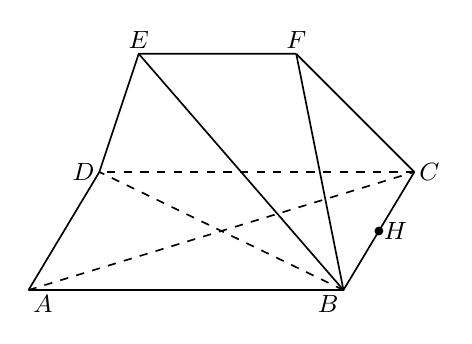
\begin{tikzpicture}[semithick, every node/.style={inner sep=1.5pt, font=\small}]
  \coordinate (A) at (0,0);
  \coordinate (B) at (4,0);
  \coordinate (C) at (4.9,1.5);
  \coordinate (D) at (0.9,1.5);
  \coordinate (E) at (1.4,3.0);
  \coordinate (F) at (3.4,3.0);
  \coordinate (H) at (4.45,0.75);

  \draw (A) -- (B) -- (C);
  \draw (A) -- (D) -- (E) -- (F) -- (E);
  \draw (F) -- (C);
  \draw (F) -- (B);
  \draw (E) -- (B);
  \draw[dashed] (C) -- (D);
  \draw[dashed] (A) -- (C);
  \draw[dashed] (B) -- (D);

  \fill (H) circle (1.6pt);
  \node[below right] at (A) {$A$};
  \node[below left] at (B) {$B$};
  \node[right] at (C) {$C$};
  \node[left] at (D) {$D$};
  \node[above] at (E) {$E$};
  \node[above] at (F) {$F$};
  \node[right] at (H) {$H$};
\end{tikzpicture}
